%%%%%%%%%%%%%%%%%%%%%%%%%%%%%%%%%%%%%%%%%%%%%%%%%%%
%% P3: Phenomenology of Particle Physics                         
%%
%% Author:  André Rubbia                   		 
%%
%% Figure 13.3 The center-of-mass energy squared normalized differential cross-sections for basic QED processes.
%%
%% This work is licensed under the Creative Commons Attribution 4.0 International License. 
%% To view a copy of this license, visit http://creativecommons.org/licenses/by/4.0/ or 
%% send a letter to Creative Commons, PO Box 1866, Mountain View, CA 94042, USA.
%%
%%%%%%%%%%%%%%%%%%%%%%%%%%%%%%%%%%%%%%%%%%%%%%%%%%%

\documentclass[a4paper,10pt]{article}

\usepackage[T1]{fontenc}
\usepackage[utf8]{inputenc}
\usepackage{lmodern}
\usepackage[labelfont=bf]{caption}
\usepackage{upgreek}

\usepackage{tikz}
\usepackage{pgfplots}
\pgfplotsset{compat=1.17}
\usepgfplotslibrary{ternary}
\usepgfplotslibrary{fillbetween}
\usepgfplotslibrary{external}

\usepackage{braket}

\def\d{\mathrm{d}}

\begin{document}

%%%%%%%%%%%%%%%%% FIGURE %%%%%%%%%%%%%%%%%%%%%%%%%%%%%%%%%%
\begin{figure}[htb]
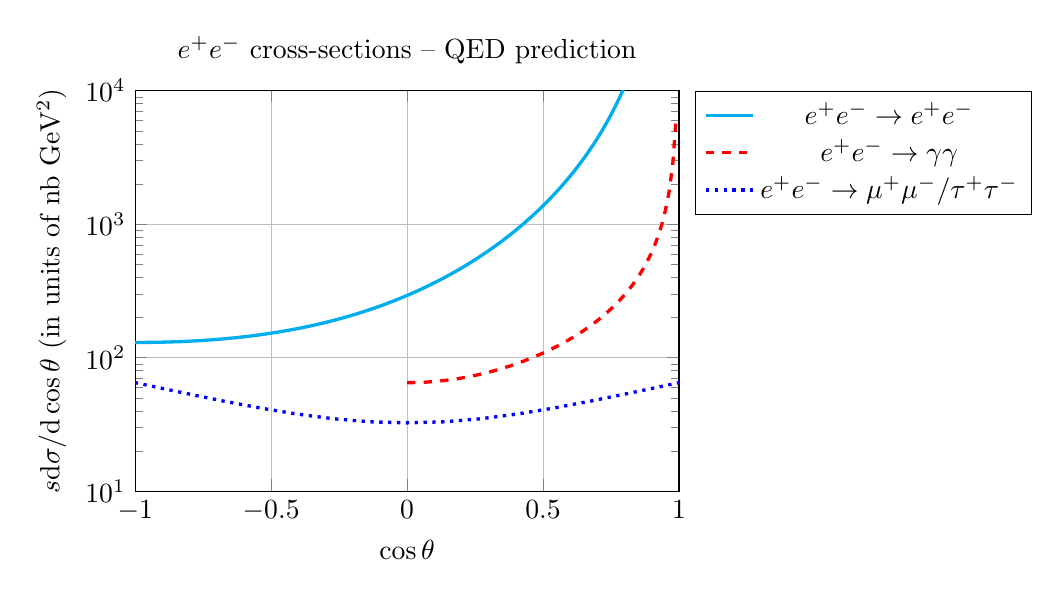
\begin{tikzpicture}[scale=1]
\begin{semilogyaxis}[
	width=0.7\textwidth,
	height=0.55\textwidth,
        title=$e^+e^-$ cross-sections -- QED prediction,
        xlabel={$\cos\theta$},
        ylabel={$s\d\sigma/\d\cos\theta$ (in units of nb GeV$^2$)},
        xmin=-1, xmax=1,
        ymin = 1e1, ymax=1e4,
        minor y tick num=1,
        grid = major,
        legend entries={
        $e^+e^-\rightarrow e^+e^-$,
         $e^+e^-\rightarrow \gamma\gamma$,
       $e^+e^-\rightarrow \mu^+\mu^-/\tau^+\tau^-$
        },
        legend style={legend pos = outer north east}
    ]
        \addplot [cyan,domain=-1:0.95, samples=75,no marks, very thick] {1e6*(1/137^2)*3.14*0.389*(3+x^2)^2/(2*(x-1)^2};
        \addplot [red,domain=0:0.99, samples=75,no marks, very thick, dashed] {1e6*(1/137^2)*3.14*0.389*(1+x^2)/(1-x^2)};
        \addplot [samples=75,blue, ,no marks, very thick, dotted] {1e6*(1/137^2)*3.14*0.389*(1+x^2)/2};
%%%        \node[blue] at (axis cs: 0,1.25) {$e^+e^-\rightarrow\ell^+\ell^-$};
\end{semilogyaxis}
\end{tikzpicture}
\caption{The center-of-mass energy squared normalized differential cross-sections $s\frac{\d\sigma}{\d\cos\theta}$ for
$e^+e^-\rightarrow e^+e^-$,
$e^+e^-\rightarrow \mu^-\mu^+$ or
$\tau^-\tau^+$, and
$e^+e^-\rightarrow \gamma\gamma$. Note the  logarithmic vertical scale.}
\end{figure}
%%%%%%%%%%%%%%%%% END FIGURE %%%%%%%%%%%%%%%%%%%%%%%%%%%%%%
%

\end{document}
